\documentclass[a4paper,10pt]{article}
%\usepackage[utf8x]{inputenc}

% Lay out packages
\usepackage[margin=3cm]{geometry}
\usepackage[utf8]{inputenc}
\usepackage{mathpazo}

\usepackage{amsmath}
\usepackage{graphicx}

% Dutch style of paragraph formatting, i.e. no indents. 
\setlength{\parskip}{1.3ex plus 0.2ex minus 0.2ex}
\setlength{\parindent}{0pt}

%opening
\title{Computer Vision Assignment 1: Filtering}
\author{Robrecht Jurriaans (5887380), Taco Cohen (6394590)}

\begin{document}

\maketitle

\section{Gaussian Filters}

\subsection{1D Gaussian Filter}
We implemented the 1D Gaussian in \verb+gaussian.m+.

\subsection{Convolving an image with a 2D Gaussian}


\subsection{Comparing with Matlab's Gaussian Filter}
\begin{figure}[ht]
\begin{minipage}[b]{0.45\linewidth}
\centering
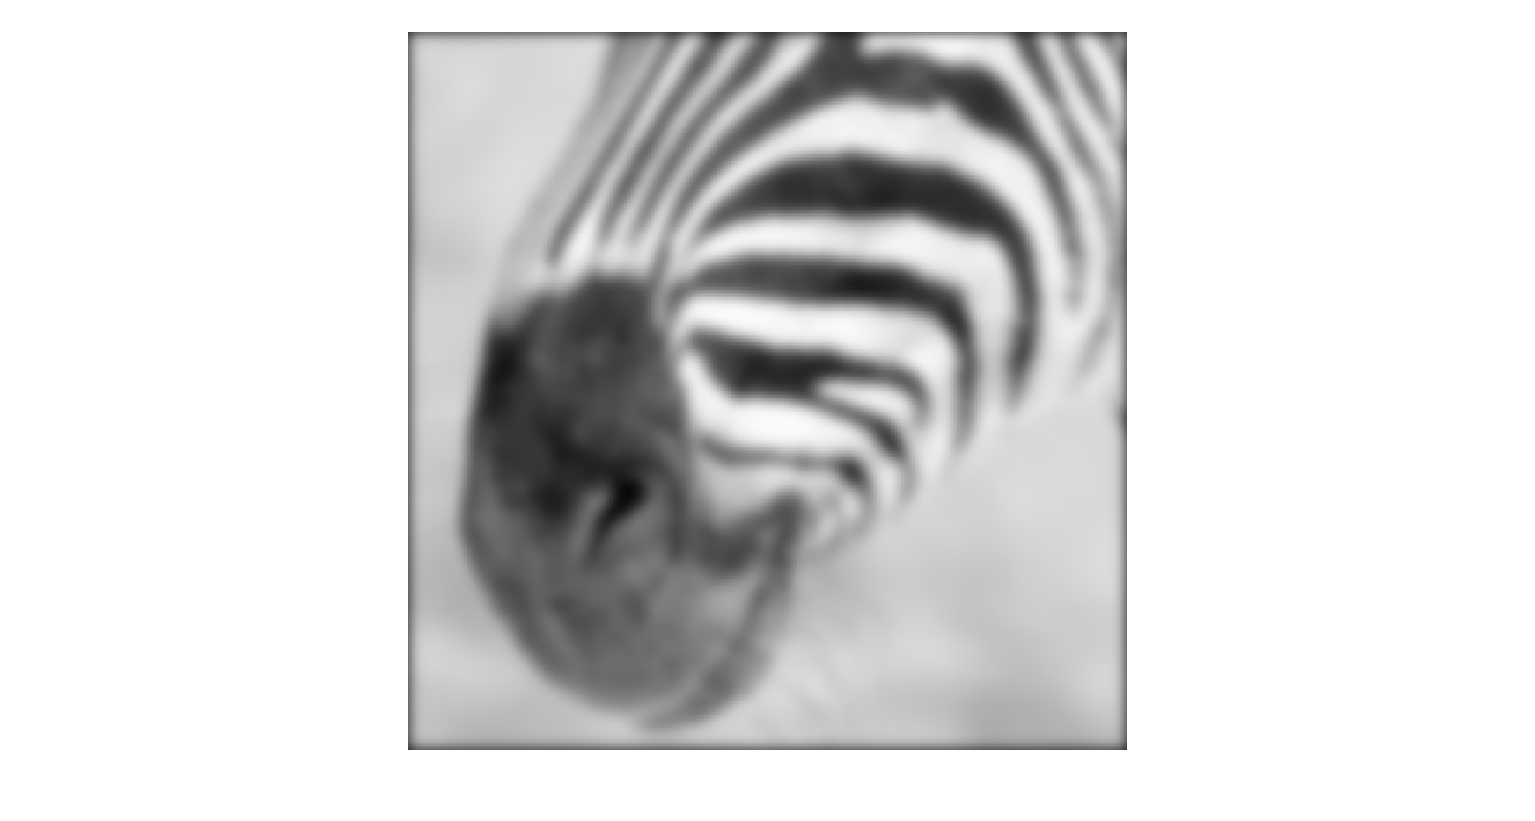
\includegraphics[width=\textwidth]{zebra_img/matlabfilter}
\caption{Original Matlab Filter}
\end{minipage}
\hspace{0.1cm}
\begin{minipage}[b]{0.45\linewidth}
\centering
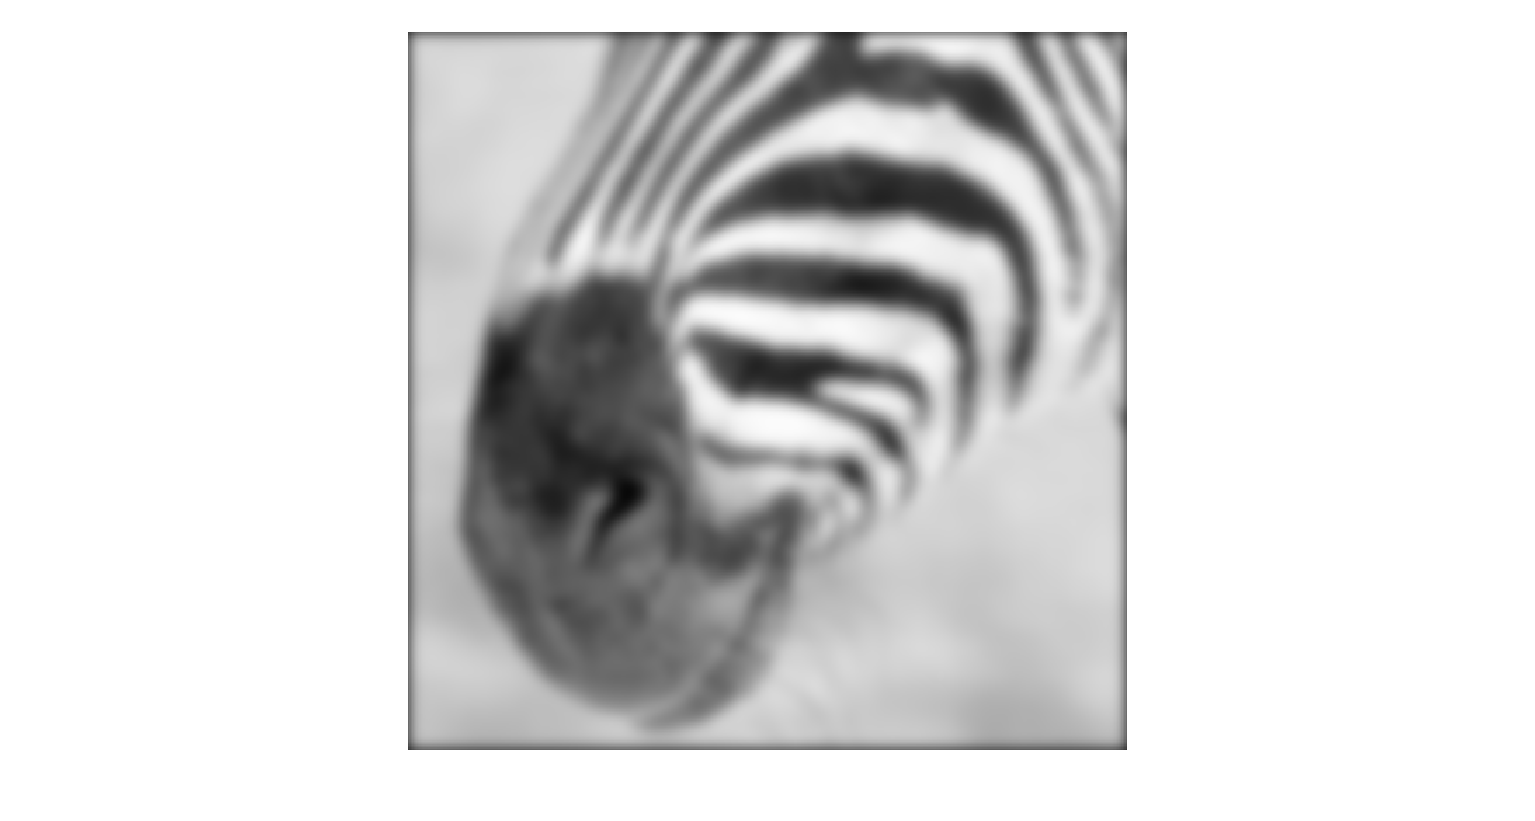
\includegraphics[width=\textwidth]{zebra_img/separatedfilter}
\caption{Filter based on separation}
\end{minipage}
\end{figure}

\subsection{Gaussian Derivative}


\subsection{Gradient Magnitude and Orientation}
\begin{figure}[ht]
\begin{minipage}[b]{0.45\linewidth}
\centering
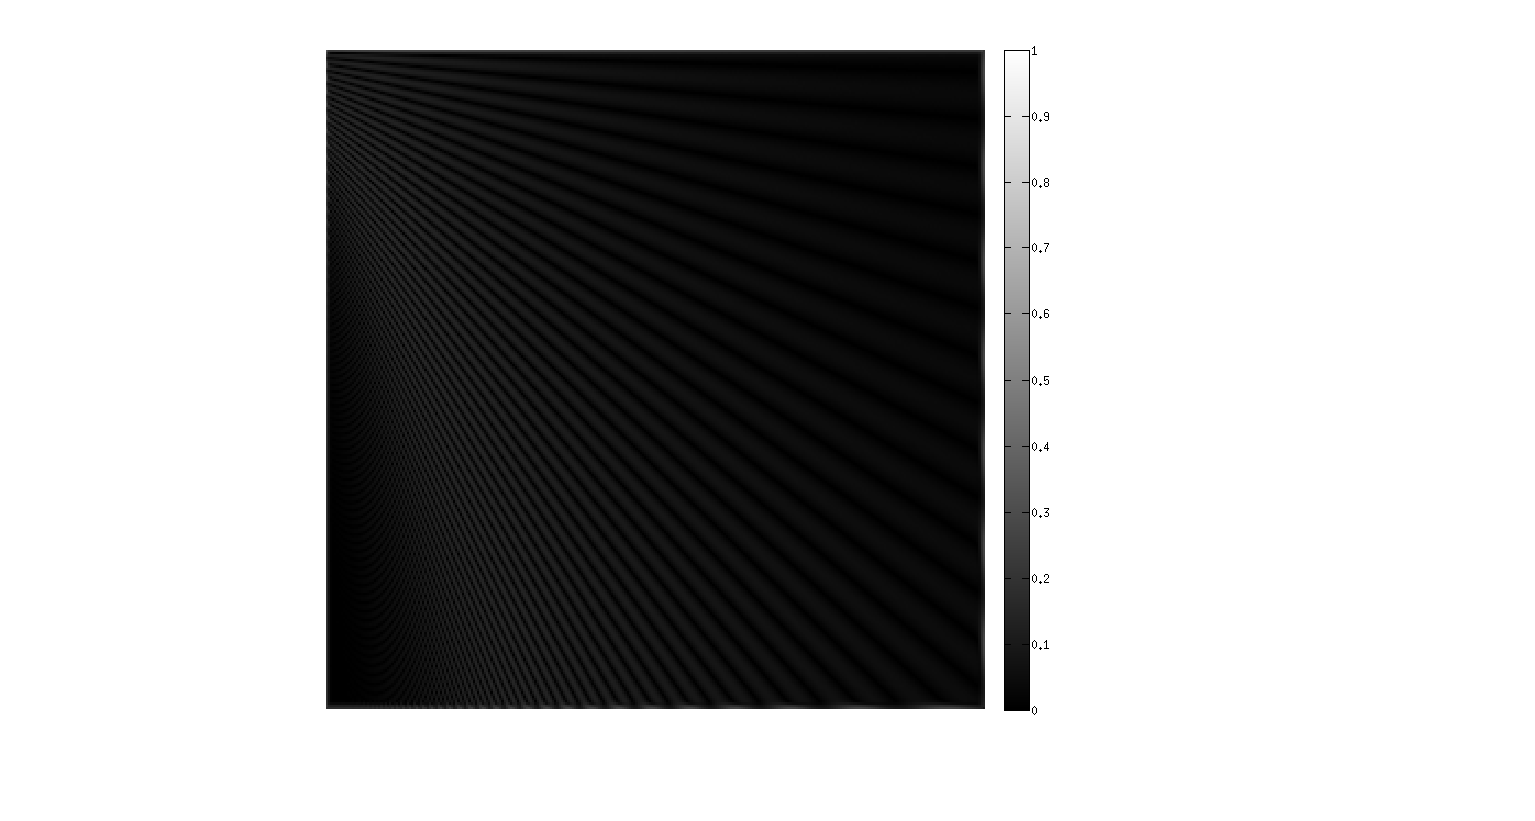
\includegraphics[width=\textwidth]{pn1_img/magnitude_sigma1}
\caption{Magnitude image for $\sigma=1$}
\end{minipage}
\hspace{0.1cm}
\begin{minipage}[b]{0.45\linewidth}
\centering
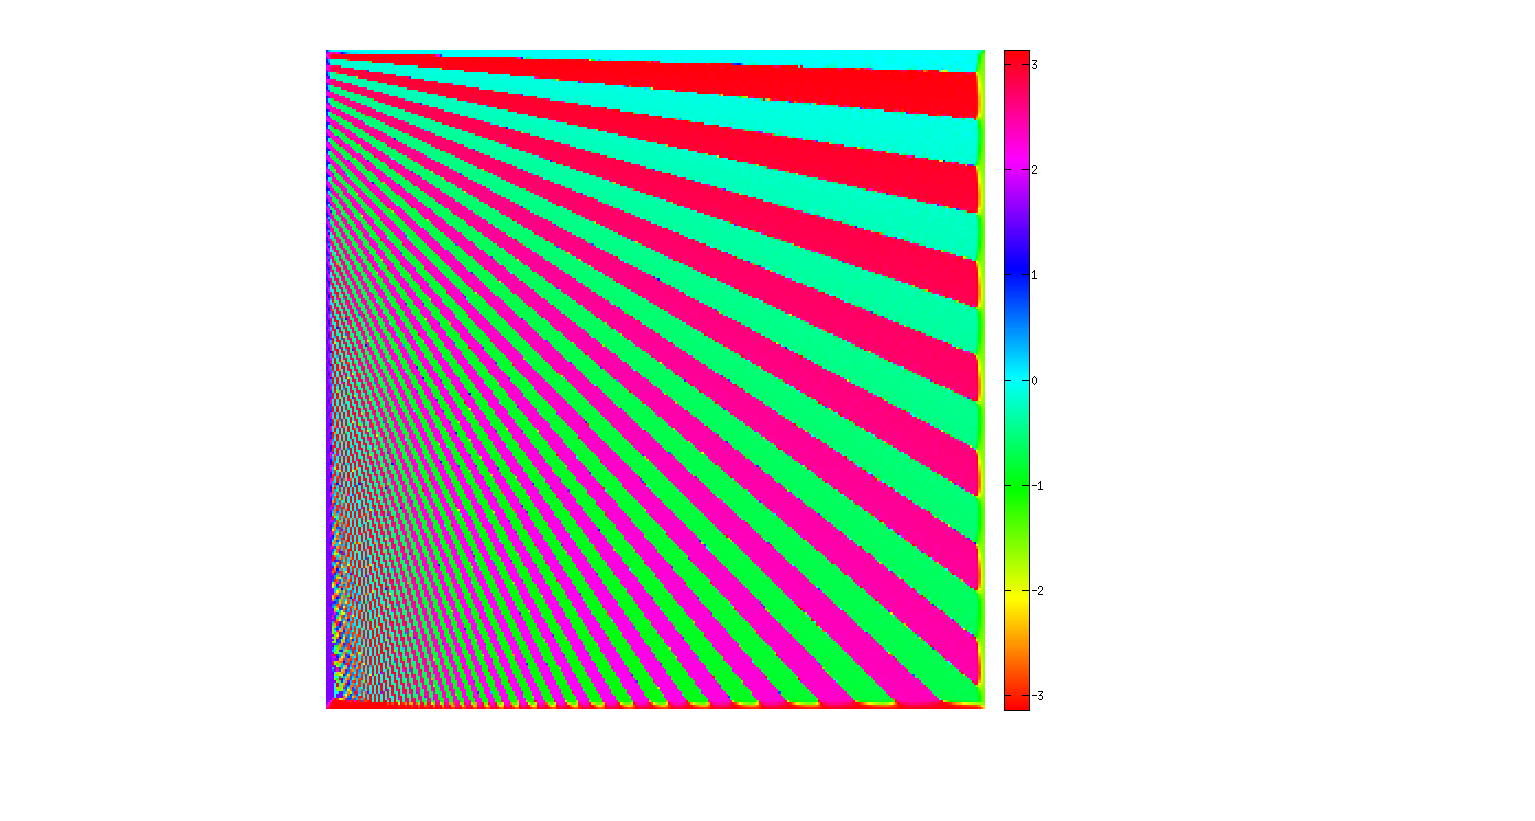
\includegraphics[width=\textwidth]{pn1_img/orientation_sigma1}
\caption{Orientation image for $\sigma=1$}
\end{minipage}
\end{figure}

\begin{figure}[ht]
\begin{minipage}[b]{0.45\linewidth}
\centering
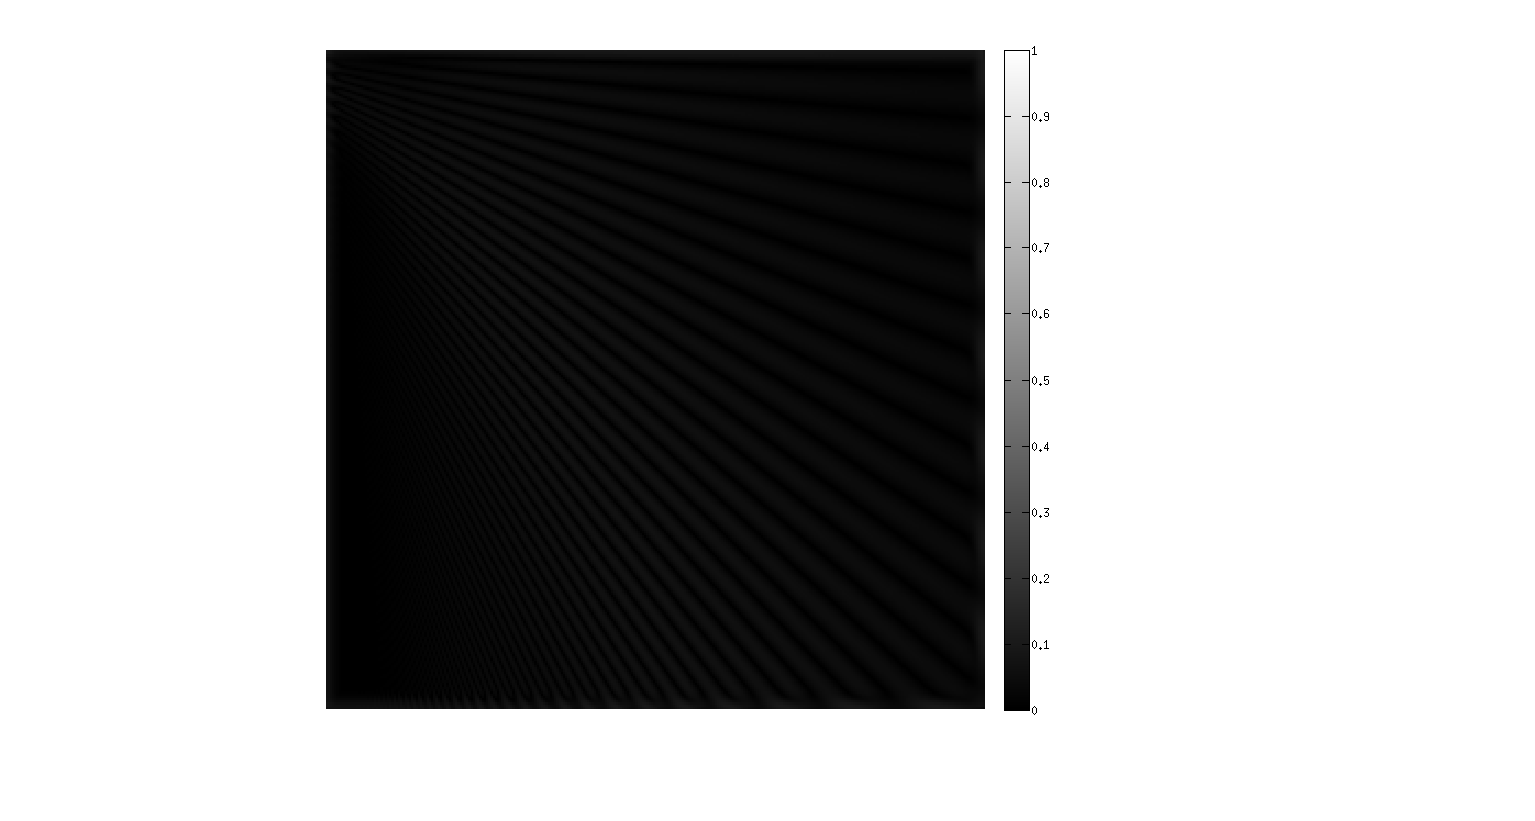
\includegraphics[width=\textwidth]{pn1_img/magnitude_sigma3}
\caption{Magnitude image for $\sigma=3$}
\end{minipage}
\hspace{0.1cm}
\begin{minipage}[b]{0.45\linewidth}
\centering
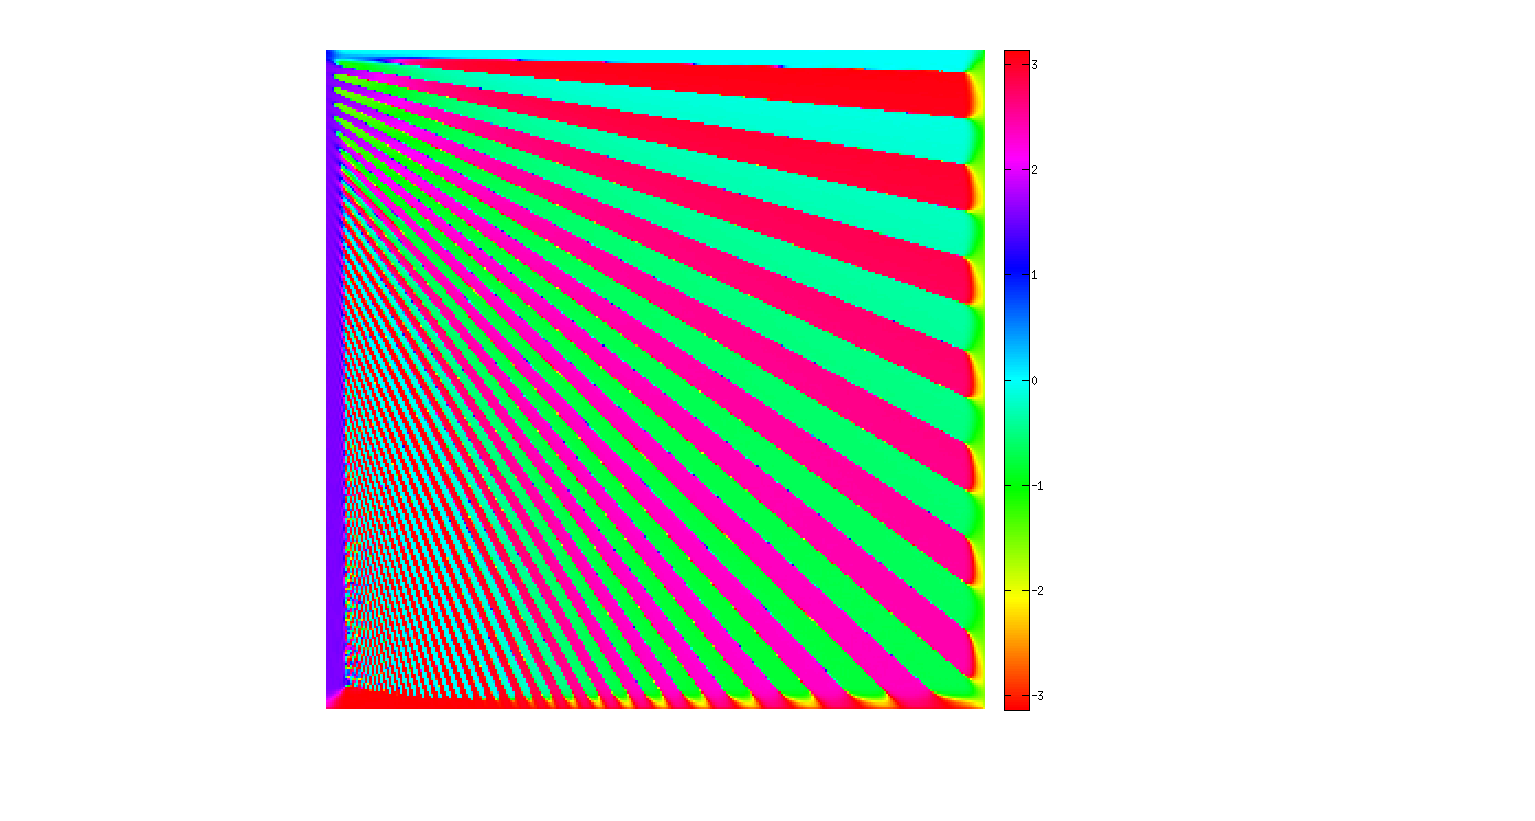
\includegraphics[width=\textwidth]{pn1_img/orientation_sigma3}
\caption{Orientation image for $\sigma=3$}
\end{minipage}
\end{figure}

\begin{figure}[ht]
\begin{minipage}[b]{0.45\linewidth}
\centering
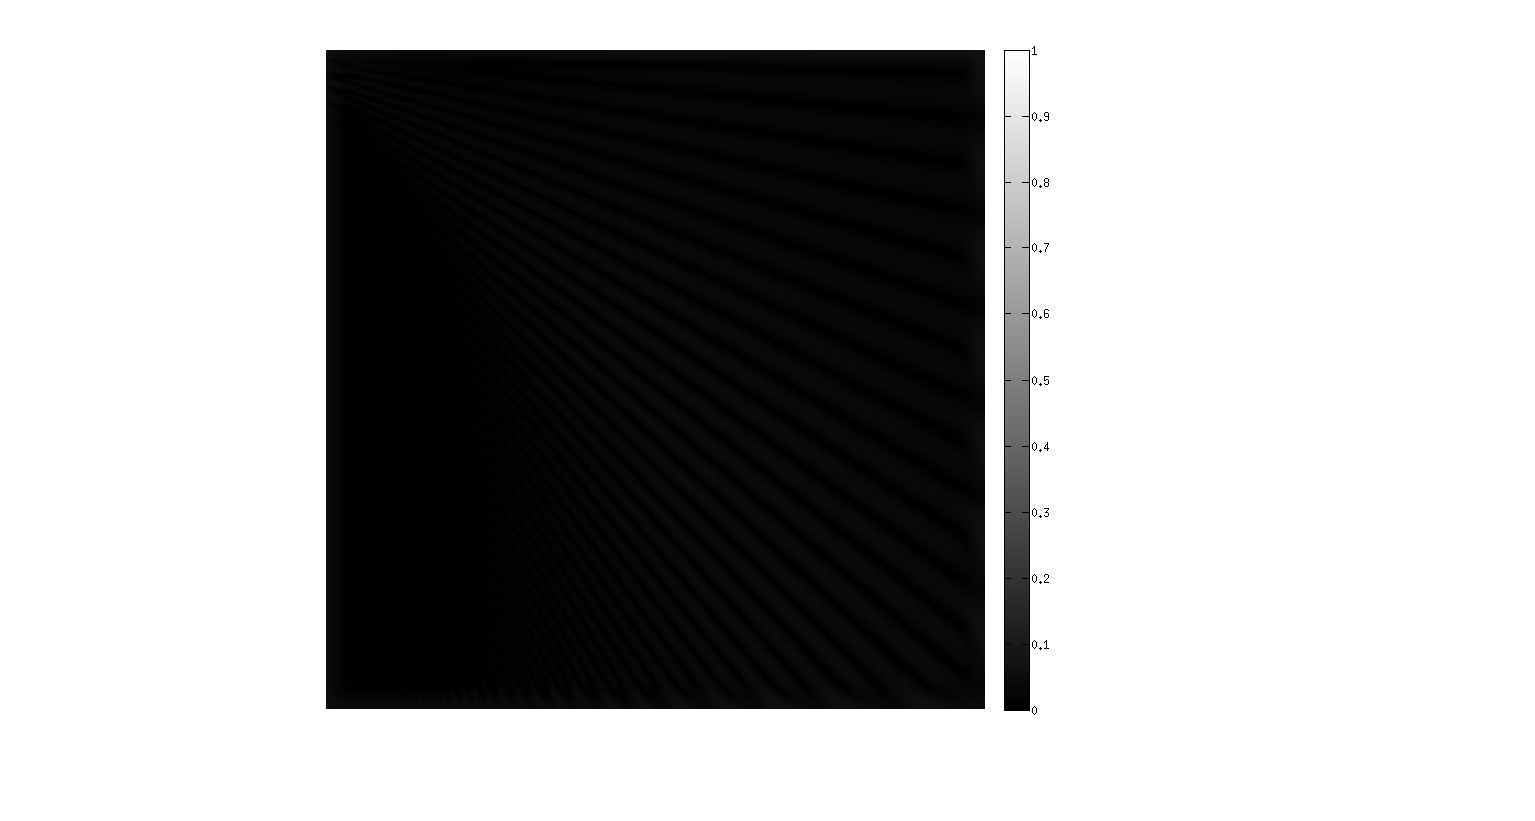
\includegraphics[width=\textwidth]{pn1_img/magnitude_sigma5}
\caption{Magnitude image for $\sigma=5$}
\end{minipage}
\hspace{0.1cm}
\begin{minipage}[b]{0.45\linewidth}
\centering
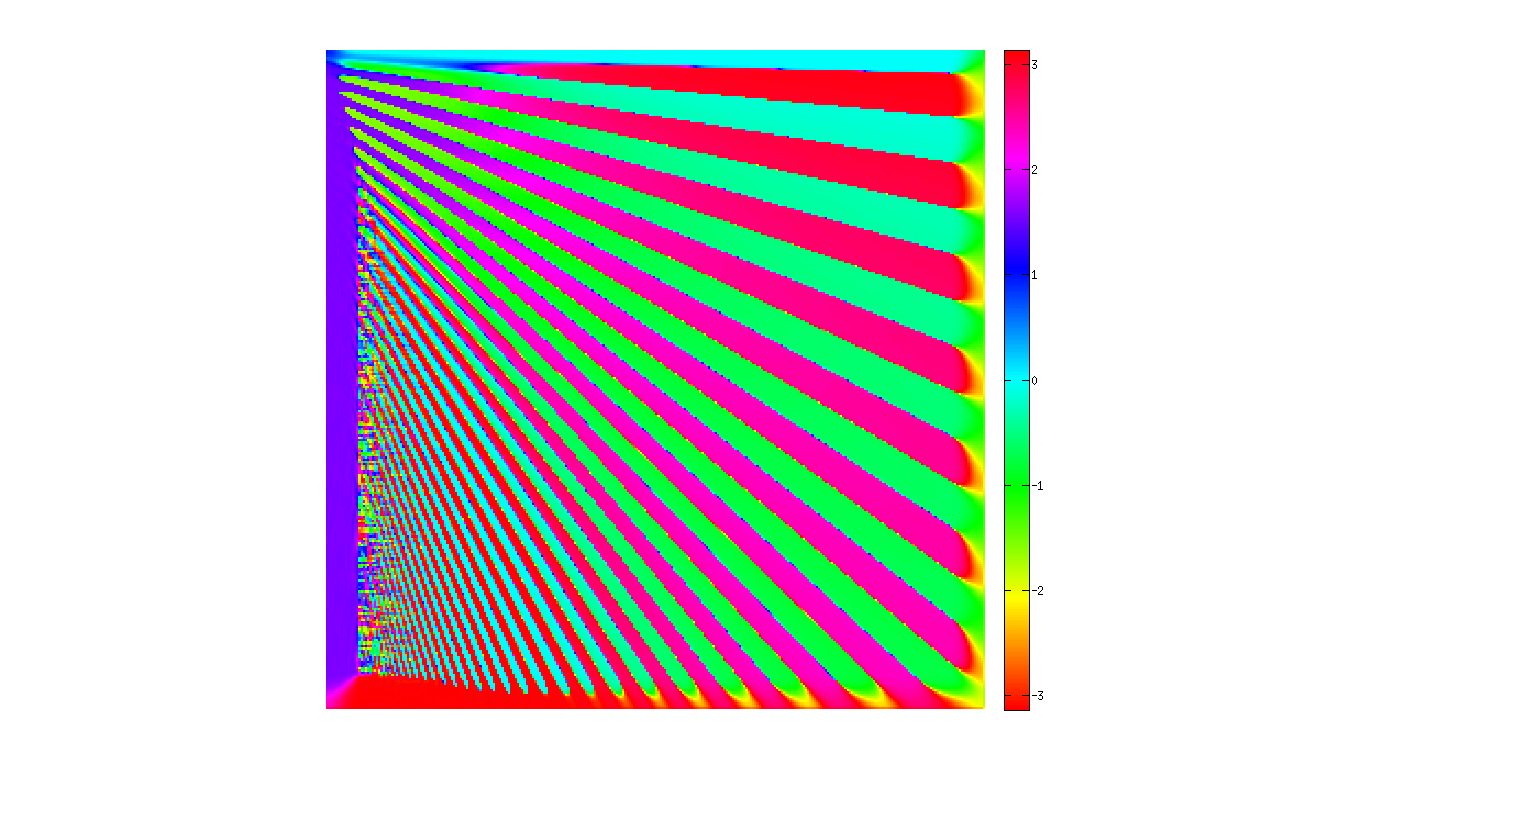
\includegraphics[width=\textwidth]{pn1_img/orientation_sigma5}
\caption{Orientation image for $\sigma=5$}
\end{minipage}
\end{figure}

\begin{figure}[ht]
\begin{minipage}[b]{0.45\linewidth}
\centering
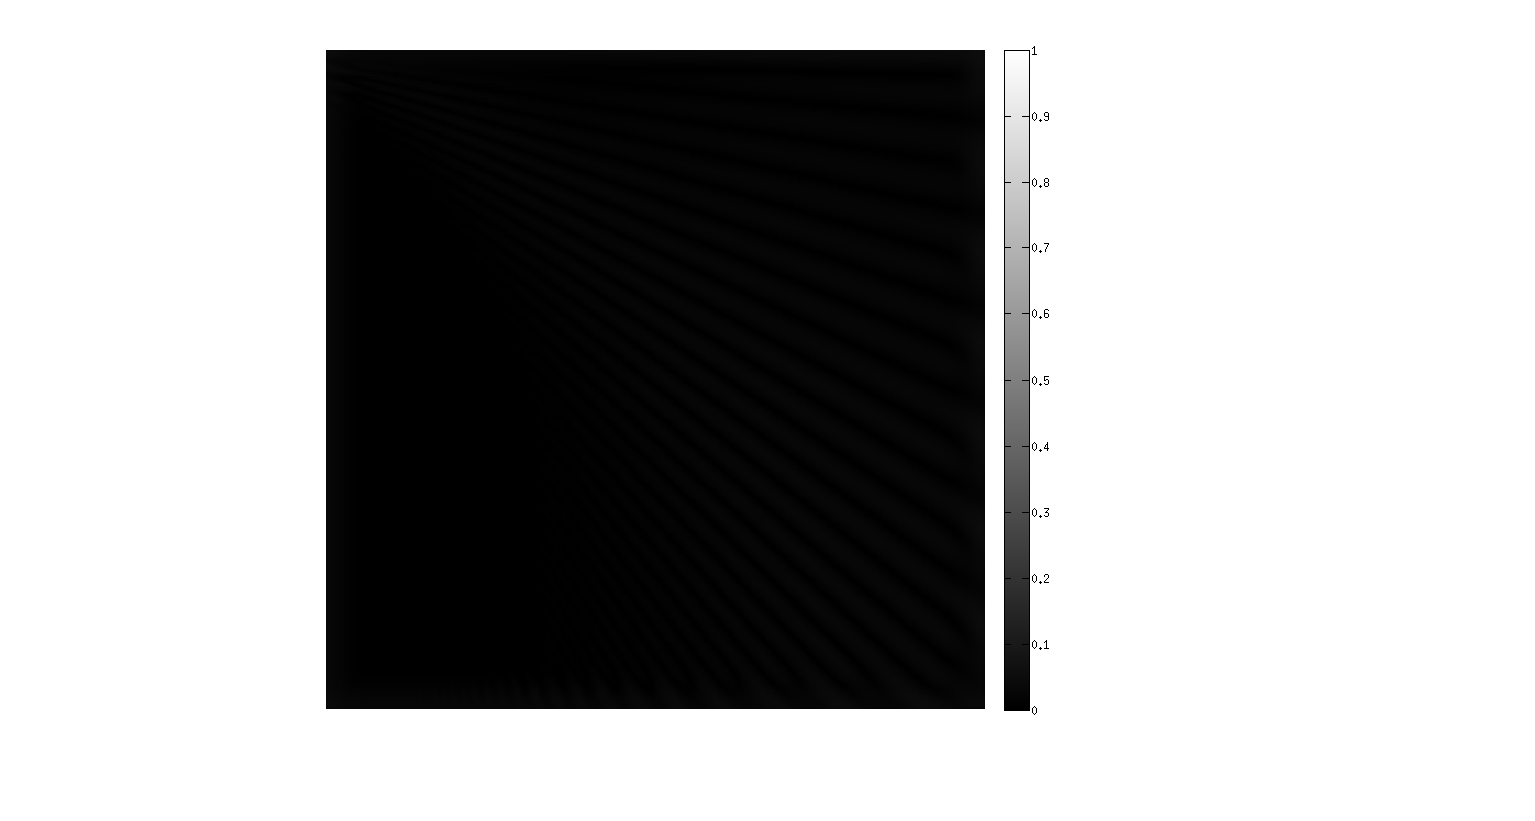
\includegraphics[width=\textwidth]{pn1_img/magnitude_sigma7}
\caption{Magnitude image for $\sigma=7$}
\end{minipage}
\hspace{0.1cm}
\begin{minipage}[b]{0.45\linewidth}
\centering
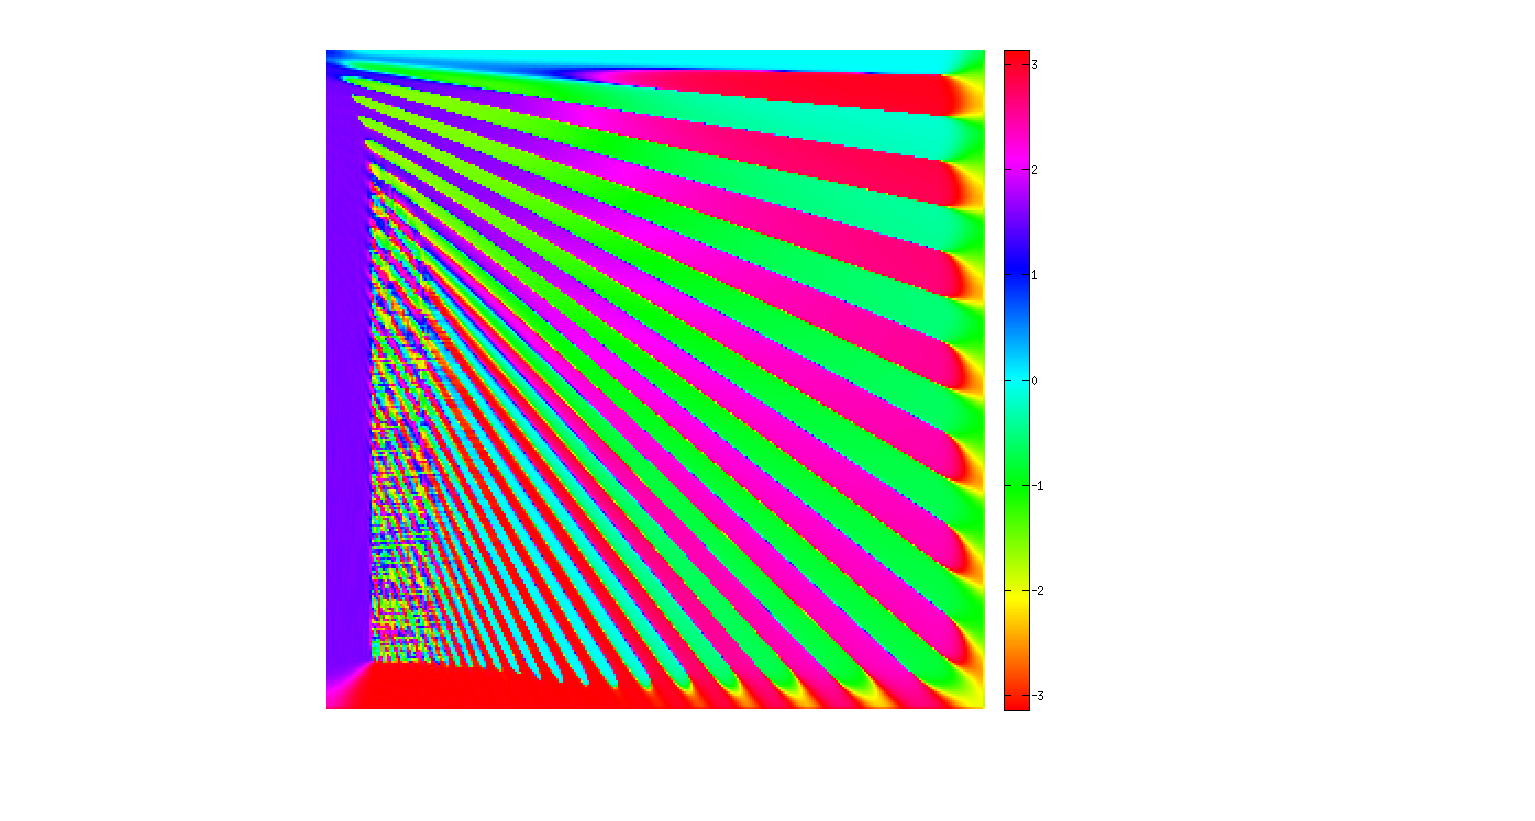
\includegraphics[width=\textwidth]{pn1_img/orientation_sigma7}
\caption{Orientation image for $\sigma=7$}
\end{minipage}
\end{figure}

\subsubsection{Quiver before my magnitude}
\begin{figure}[ht]
\centering
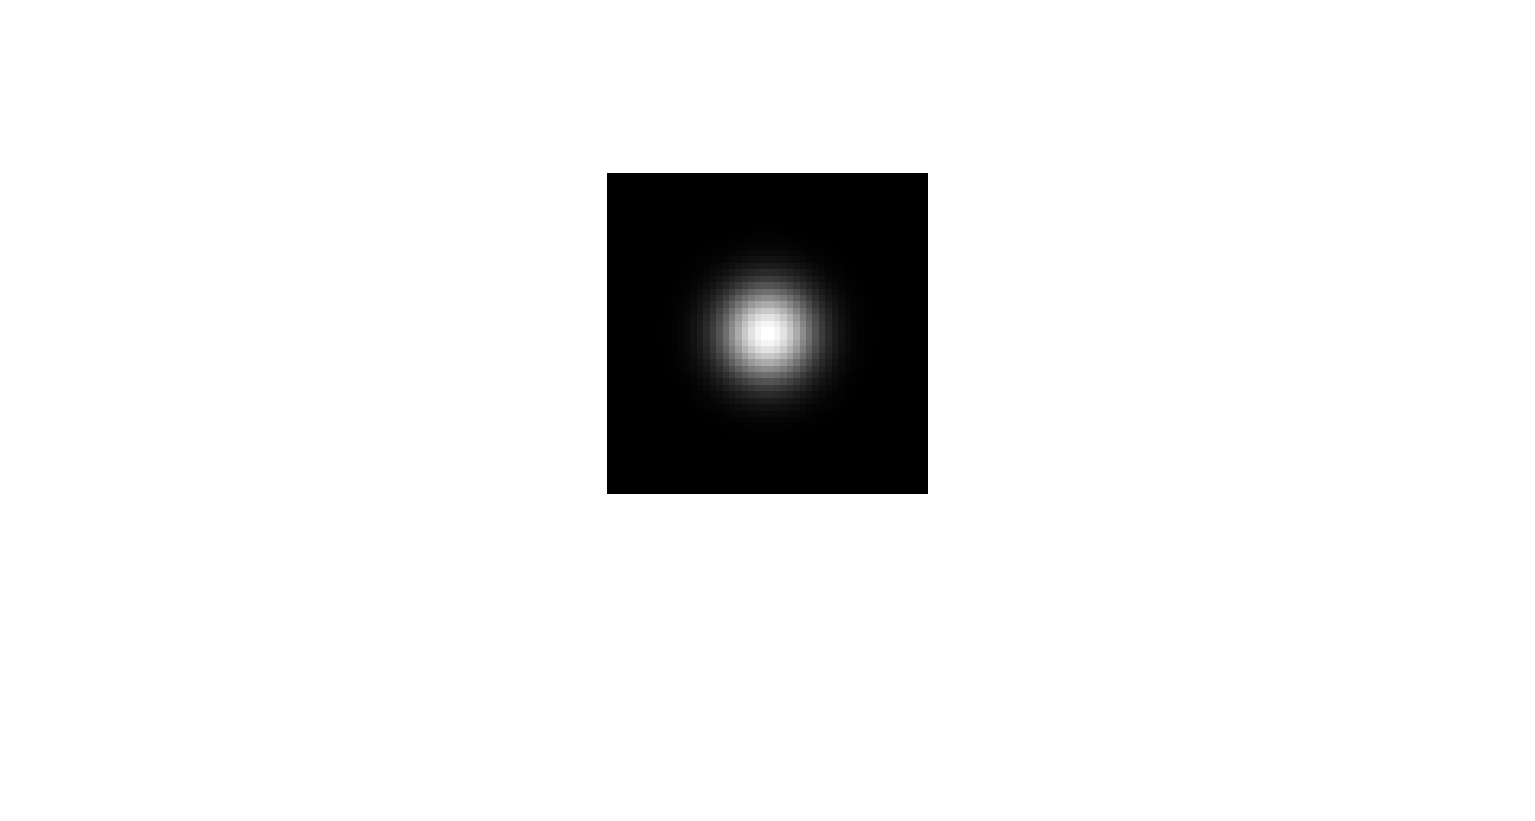
\includegraphics[width=\textwidth]{quiver_original}
\caption{Original image}
\label{fig:quiver_original}
\end{figure}
\begin{figure}[ht]
\begin{minipage}[b]{0.45\linewidth}
\centering
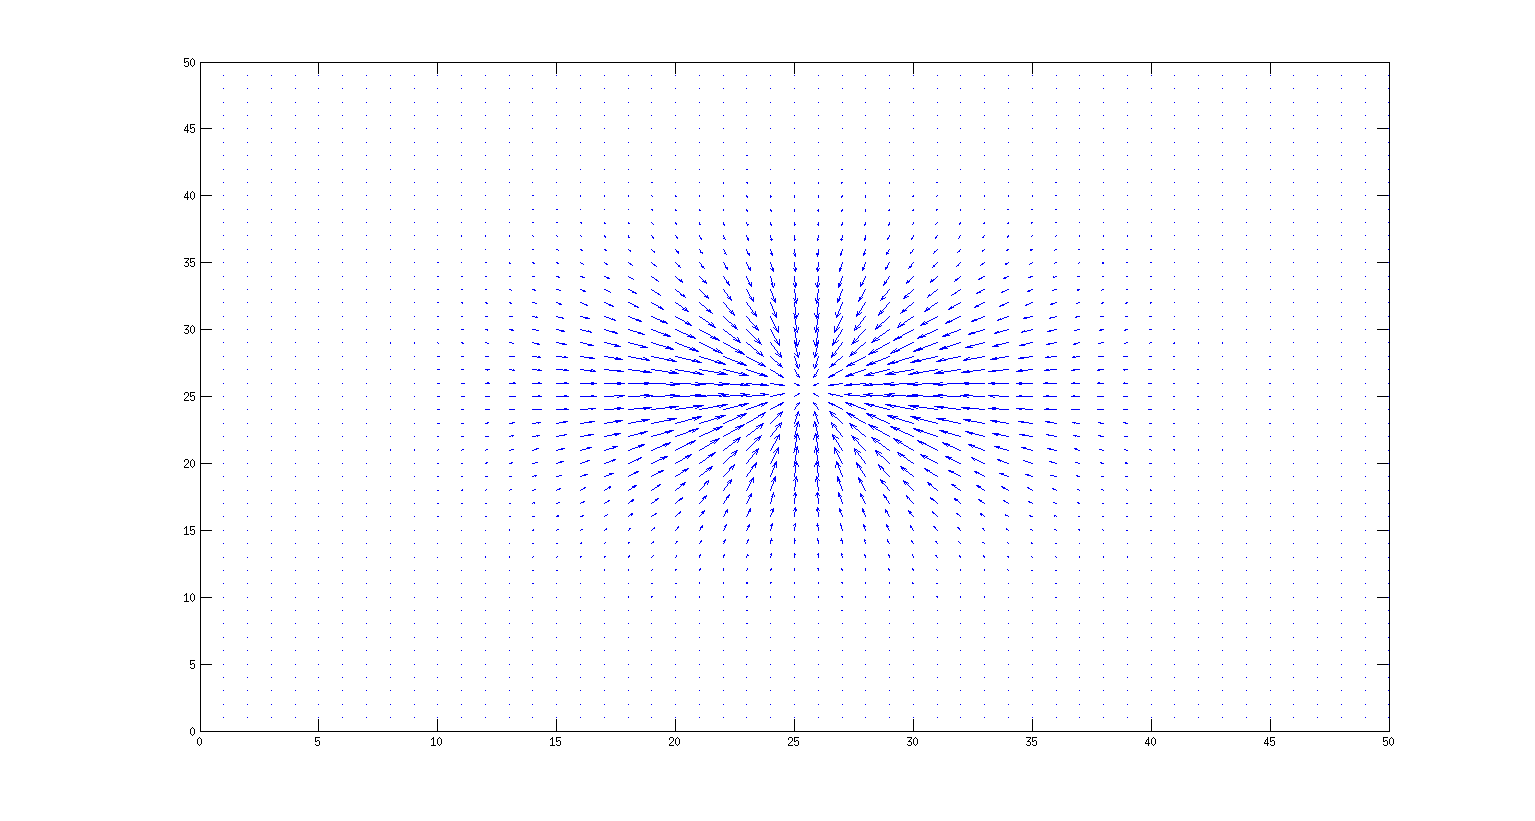
\includegraphics[width=\textwidth]{quiver_sigma1}
\caption{Gradient image for $\sigma=1$}
\end{minipage}
\hspace{0.1cm}
\begin{minipage}[b]{0.45\linewidth}
\centering
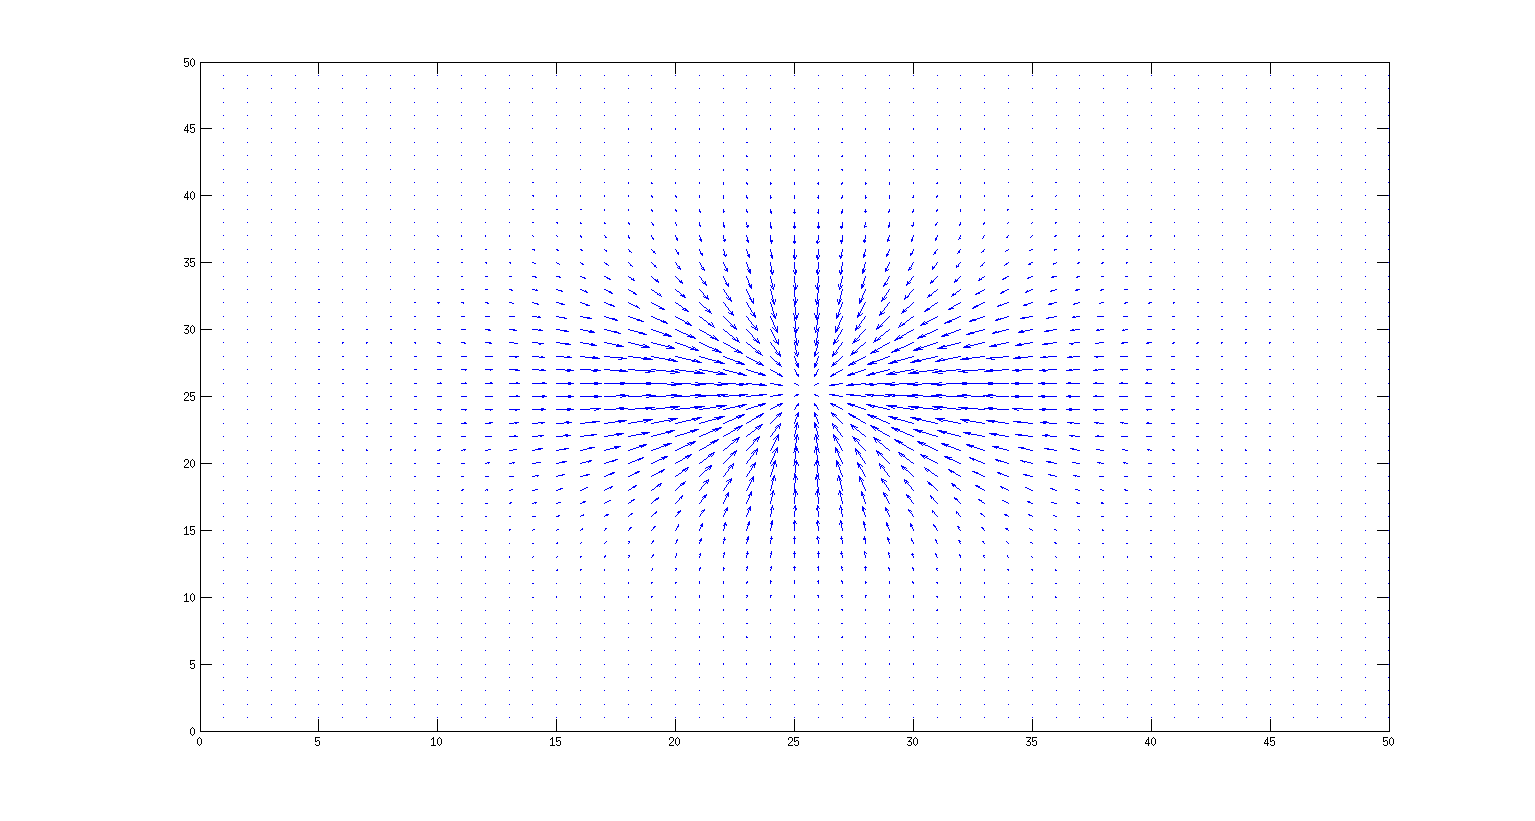
\includegraphics[width=\textwidth]{quiver_sigma3}
\caption{Gradient image for $\sigma=3$}
\end{minipage}
\end{figure}
\begin{figure}[ht]
\begin{minipage}[b]{0.45\linewidth}
\centering
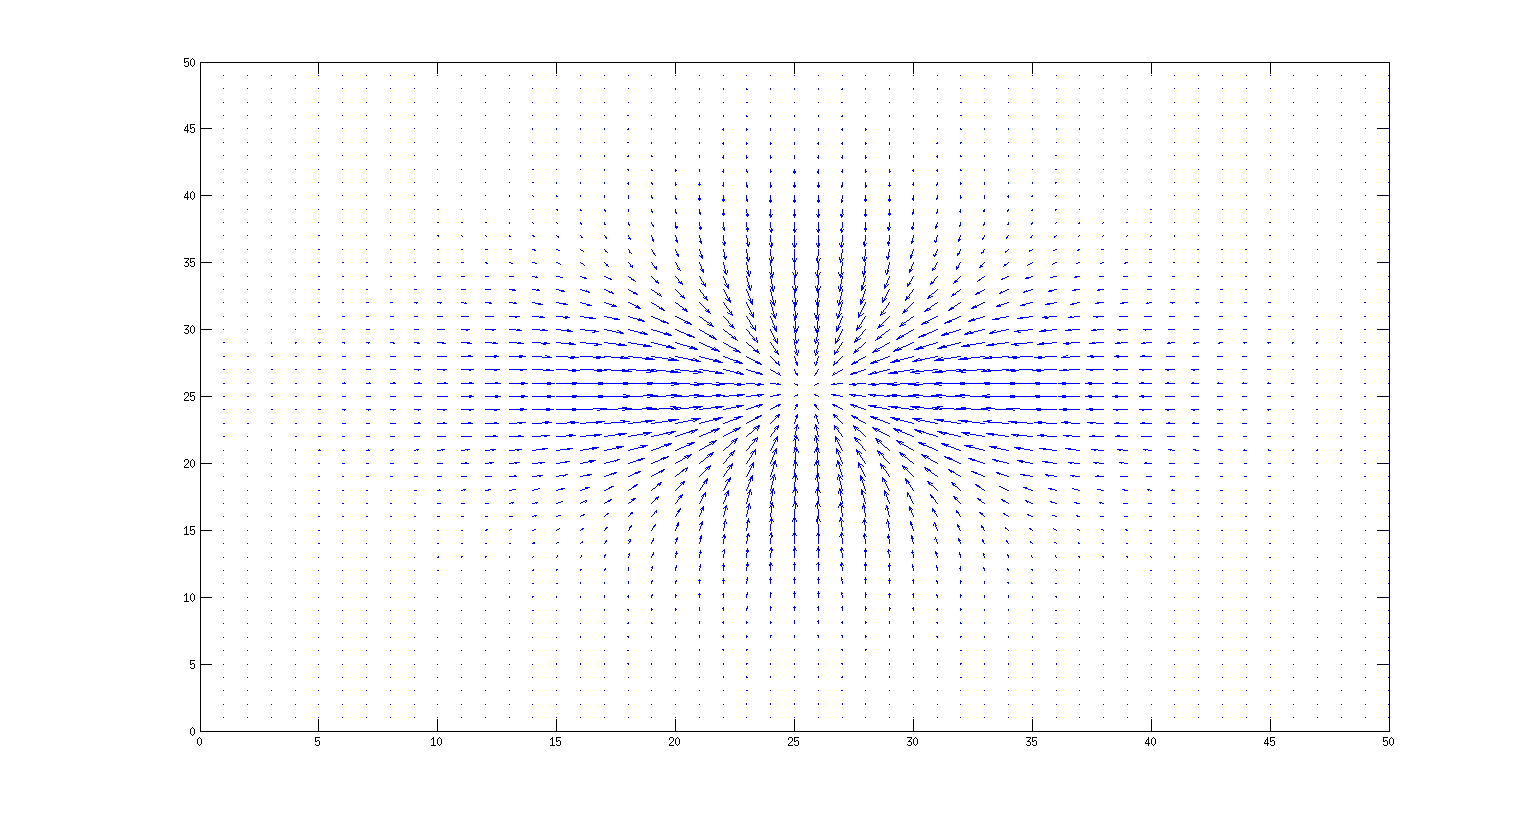
\includegraphics[width=\textwidth]{quiver_sigma5}
\caption{Gradient image for $\sigma=5$}
\end{minipage}
\hspace{0.1cm}
\begin{minipage}[b]{0.45\linewidth}
\centering
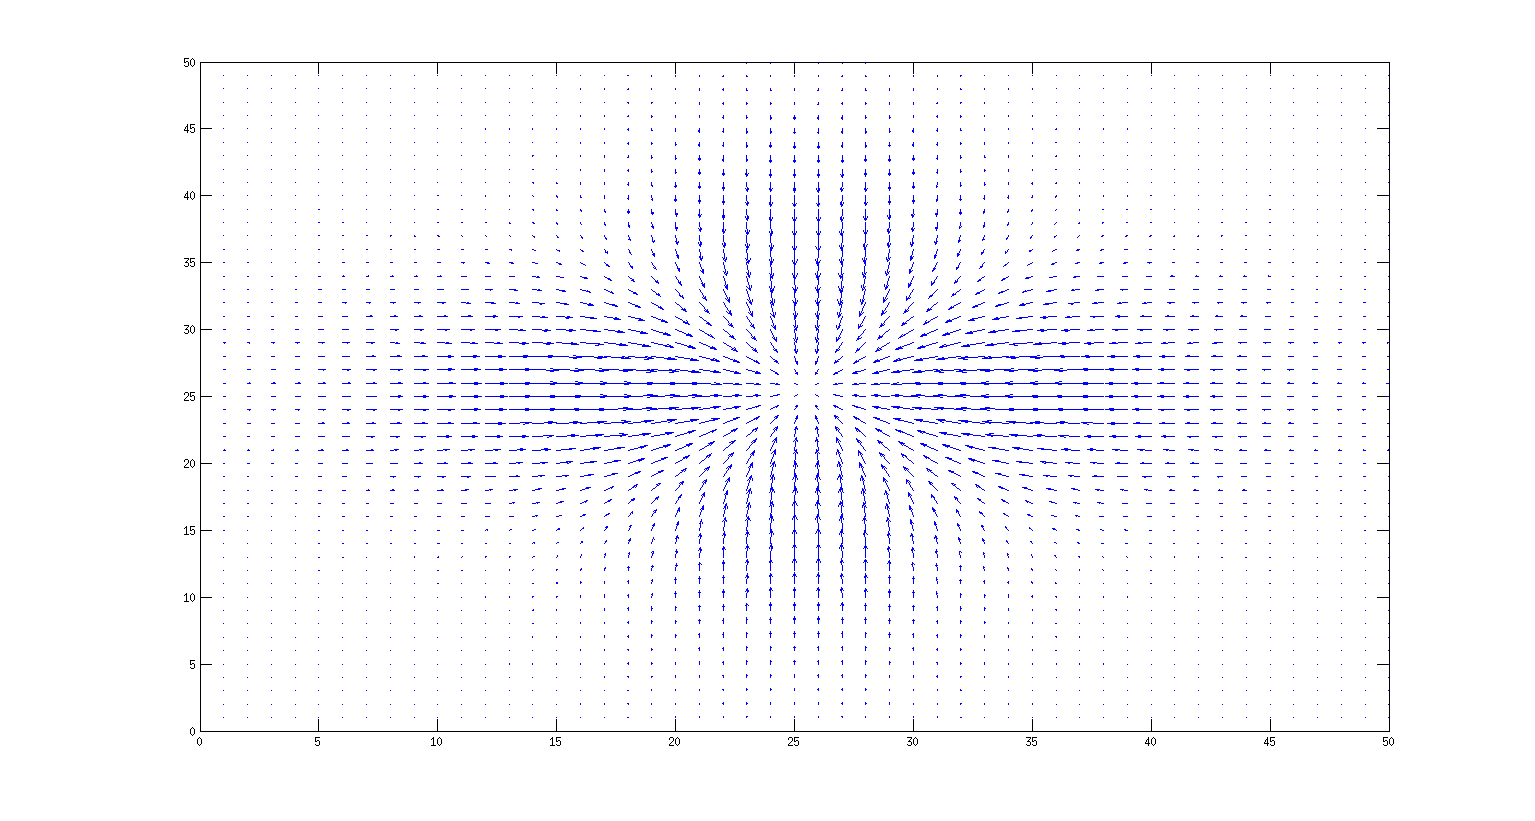
\includegraphics[width=\textwidth]{quiver_sigma7}
\caption{Gradient image for $\sigma=7$}
\end{minipage}
\end{figure}

\subsubsection{Magnitude and orientation for different $\sigma$}



\subsubsection{Threshold}
\begin{figure}[ht]
\centering
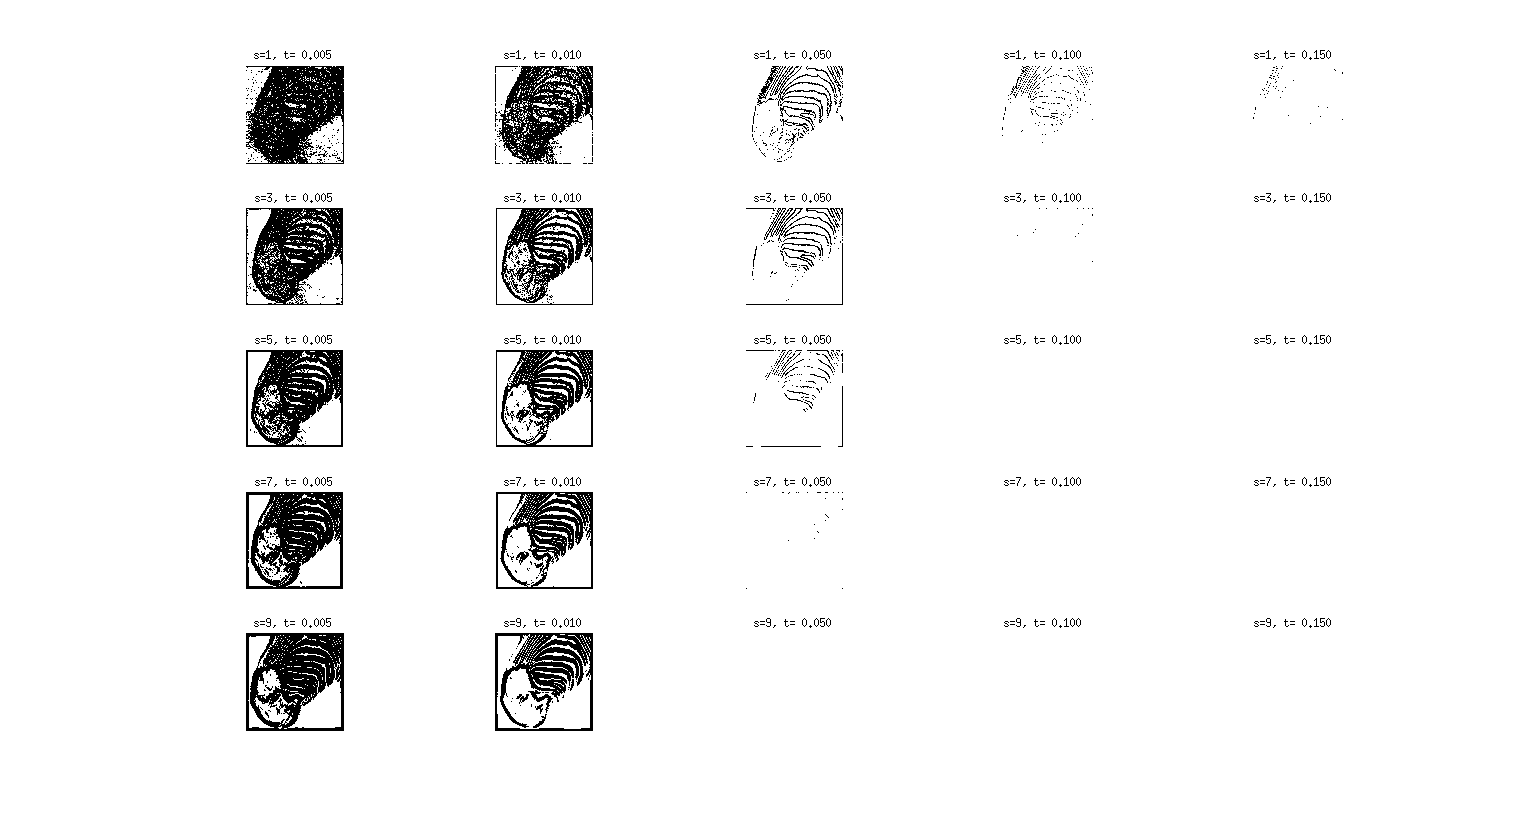
\includegraphics[width=\textwidth]{zebra_img/threshold}
\caption{Threshold images for various $\sigma$ and thresholds}
\label{fig:zebrathresh}
\end{figure}
\begin{figure}[ht]
\centering
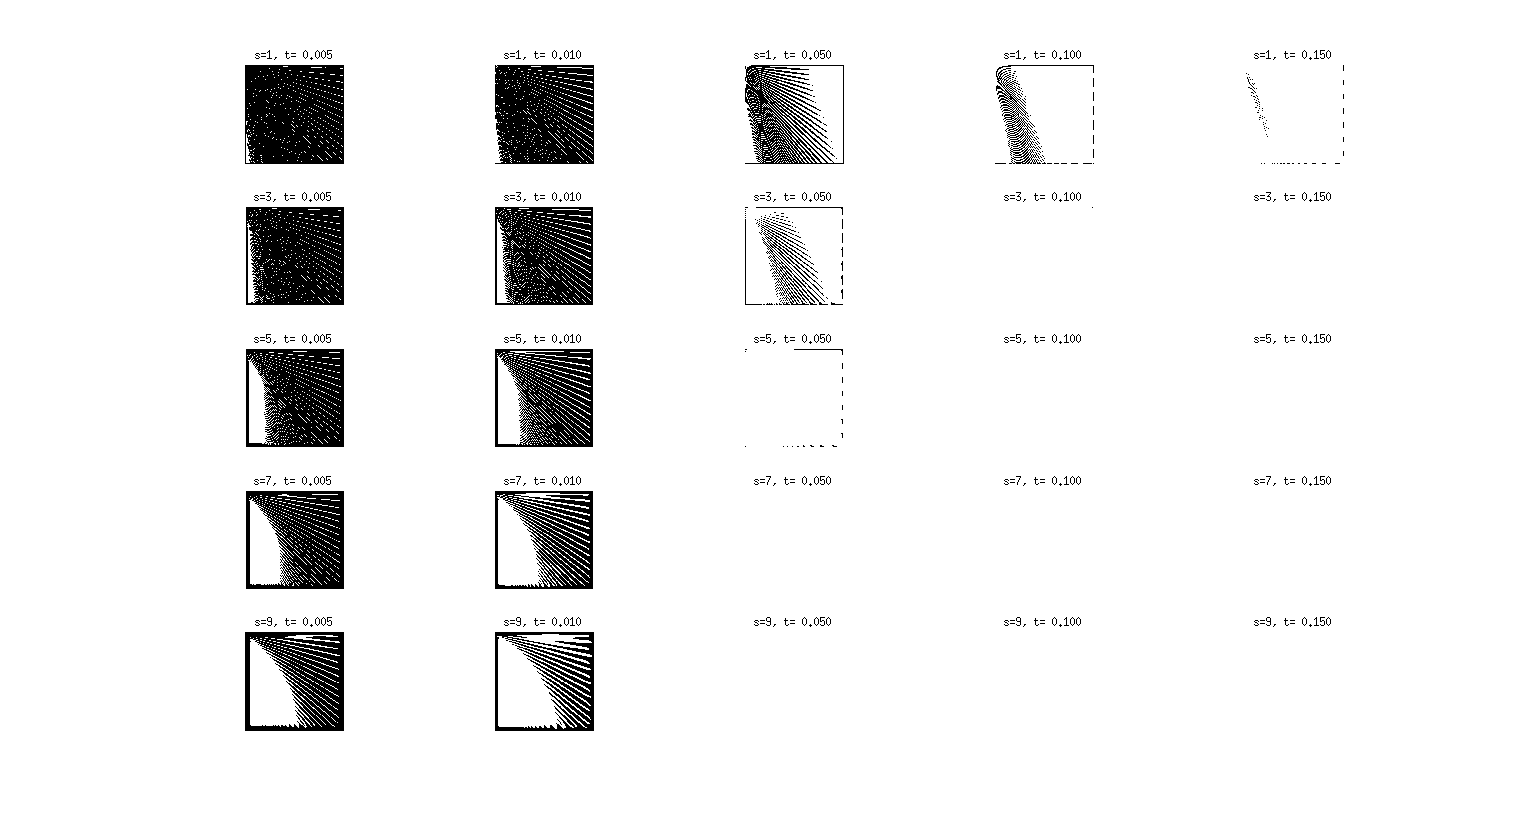
\includegraphics[width=\textwidth]{pn1_img/threshold}
\caption{Threshold images for various $\sigma$ and thresholds}
\label{fig:pn1thresh}
\end{figure}

\subsubsection{Second Order Derivative}



\subsubsection{Impulse}

\begin{figure}[ht]
\centering
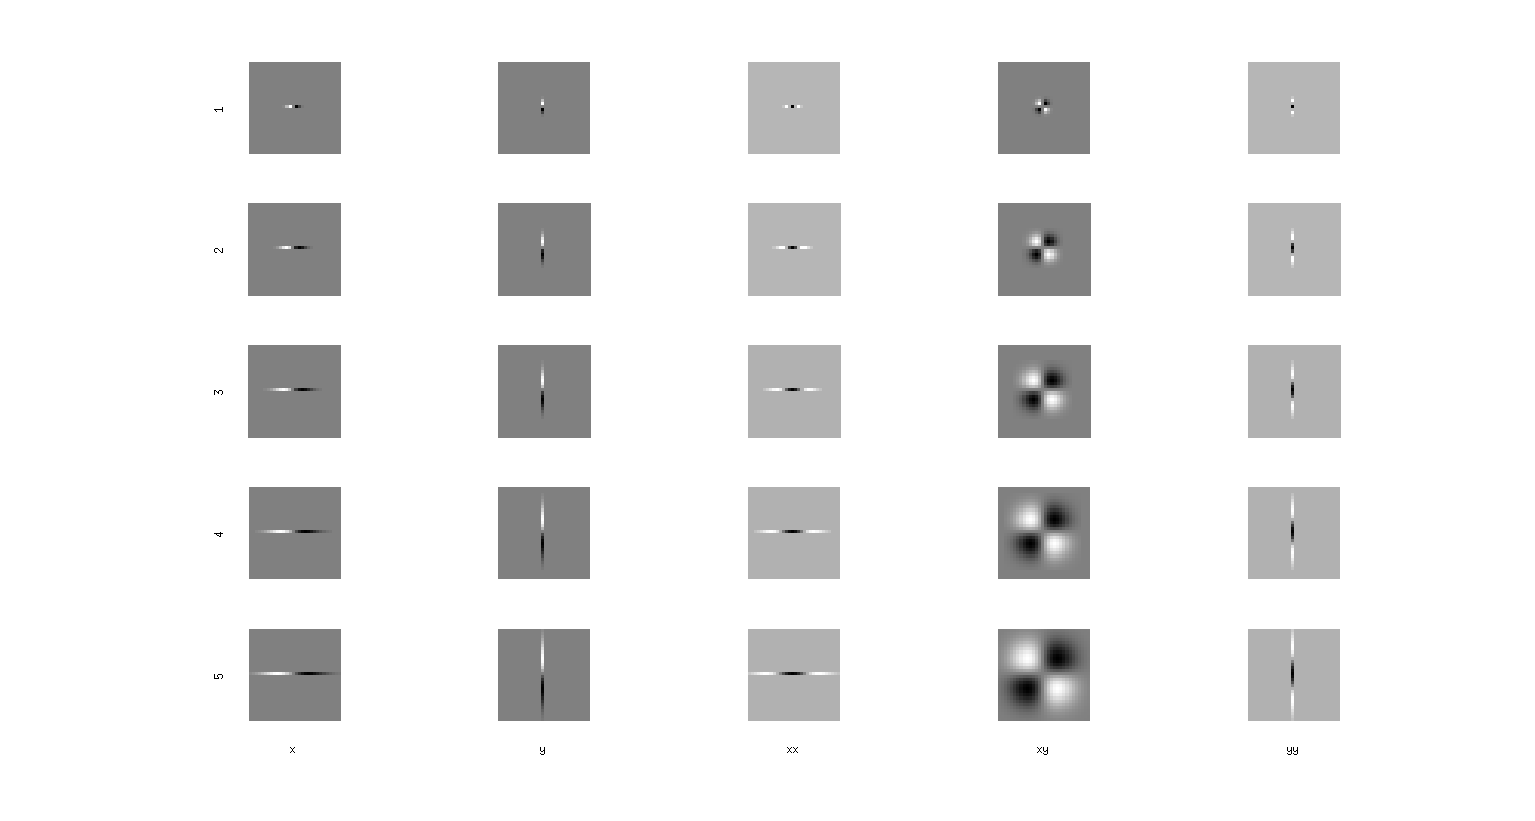
\includegraphics[width=\textwidth]{zebra_img/impulse}
\caption{30x30 impulse image convolved with various filters with $\sigma \in {1,2,3,4,5}$}
\label{fig:impulse}
\end{figure}



\subsection{Convolving an Image with a 2D Gaussian}


\end{document}
